\documentclass[11pt]{article}
\usepackage{amsmath,amsfonts,amssymb}
\usepackage{graphicx}
\usepackage{geometry} % Required for customizing margins
\geometry{margin=1in} % Sets 1-inch margins on all sides

\begin{document}

\title{ELCT 331 Control Systems Assignment 3}
\author{Jacob C. Vaught}
\date{October 8th, 2023}
\maketitle

\section*{Problem \#1}
Write the force equations of the linear translational systems shown in the Figure.
\newline
\begin{center}
    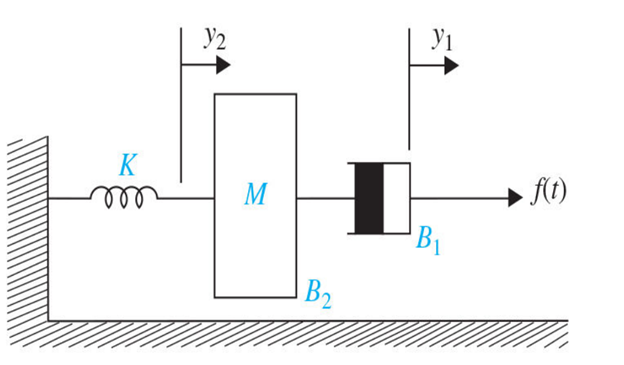
\includegraphics[width=0.8\textwidth]{hw3_p1.png}
\end{center}
\subsection*{(a) System Block Diagrams or SFGs}
Draw the system block diagrams or Signal Flow Graphs (SFGs).

\subsection*{(b) State Variables}
Define the state variables as follows:
\begin{enumerate}
    \item \( x_1 = y_1, x_2 = \frac{dy_2}{dt}, x_3 = y_1, \) and \( x_4 = \frac{dy_1}{dt} \)
    \item \( x_1 = y_2, x_2 = y_1, \) and \( x_3 = \frac{dy_1}{dt} \)
    \item \( x_1 = y_1, x_2 = y_2, \) and \( x_3 = \frac{dy_2}{dt} \)
\end{enumerate}

\subsection*{(c) State Equations and Transfer Functions}
Write the state equations. Find the transfer functions \( Y_1(s)/F(s) \) and \( Y_2(s)/F(s) \).

\subsubsection*{Solution}
For the damper, the force equation is \( B_1(\dot{y}_1 - \dot{y}_2) \).
For the spring, the force equation is \( k \cdot y_2 \).
\newline\newline
So, we have \( f = B_1(\dot{y}_1 - \dot{y}_2) \) and
\[
\ddot{y}_2 = \frac{B_1}{m} \dot{y}_1 - \frac{(B_1 + B_2)}{m} \dot{y}_2 - \frac{k}{m} y_2
\]
\begin{center}
    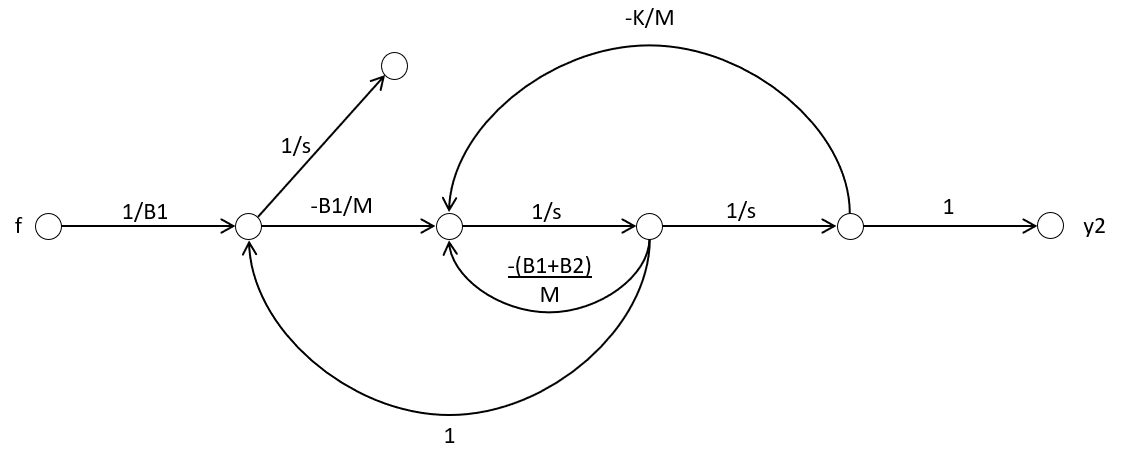
\includegraphics[width=1\textwidth]{hw3_p1sfg.png}
\end{center}
\subsubsection*{Transfer Functions}
For \( Y_2/F \):
\[
\Delta = 1 + \frac{k}{MS^2} + \frac{B_2}{MS} \quad \text{and} \quad Y_2/F = \frac{1}{MS^2+B_2S+k}
\]
\newline
For \( Y_1/F \):
\[
Y_1/F = \frac{MS^2+S(B_1+B_2)+k}{B_1S(MS^2+B_2S+k)}
\]

\subsubsection*{State Equations in Matrix Form}
Let \( x_1 = y_1, x_2 = y_2, x_3 = \dot{y}_2 \). From the force equation, we have:
\[
\begin{aligned}
\begin{pmatrix}
\dot{x}_1 \\
\dot{x}_2 \\
\dot{x}_3
\end{pmatrix}
&=
\begin{pmatrix}
0 & 0 & 1 \\
0 & 0 & 1 \\
0 & -\frac{K}{M} & -\frac{B_1}{M}
\end{pmatrix}
\begin{pmatrix}
x_1 \\
x_2 \\
x_3
\end{pmatrix}
+
\begin{pmatrix}
\frac{1}{B_1} \\
0 \\
\frac{1}{M}
\end{pmatrix} f
\end{aligned}
\]

\newpage
\section*{Problem \#2}

From the figure below, find the following:
\begin{center}
    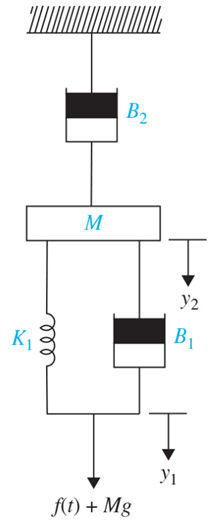
\includegraphics[width=0.2\textwidth]{hw3_p2.png}
\end{center}

\begin{enumerate}
    \item Write the force equations of the linear translational system.
    \item Draw system block diagrams.
    \item Write the state equations.
    \item Find the transfer functions \(Y_1(s)/F(s)\) and \(Y_2(s)/F(s)\). Set \(Mg = 0\) for the transfer functions.
\end{enumerate}

\subsubsection*{Solution}

\begin{center}
    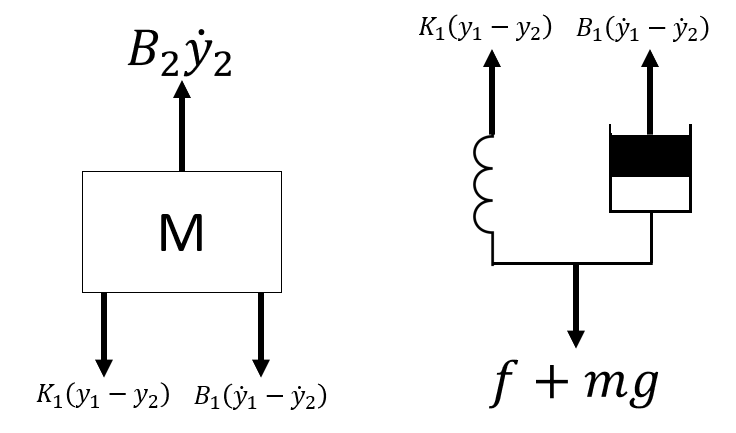
\includegraphics[width=0.5\textwidth]{hw3_p2fe.png} % Force diagram image.
\end{center}

\begin{align}
    M \ddot{y}_2 &= K_1(y_1 - y_2) + B_1(\dot{y}_1 - \dot{y}_2) - b_2 \dot{y}_2 \\
    f + Mg &= K_1(y_1 - y_2) + B_1(\dot{y}_1 - \dot{y}_2)
\end{align}


\subsubsection*{Rewriting the force equation}

\begin{align}
    y\dot_1 &= \frac{f+mg}{B_1} + y\dot_2 - \frac{K_1}{B_1} y_1 + \frac{K_1}{B_1} y_2 \\
    y\ddot_2 &= \frac{B_1}{m} y\dot_1 - \frac{B_1+B_2}{M} y\dot_2 + \frac{K_1}{M} y_1 - \frac{K_1}{M} y_2
\end{align}

\subsubsection*{Taking the Laplace transform}

\begin{align}
    SY_1 &= \frac{f+mg}{B_1} + \left( \frac{B_1S+K_1}{B_1} \right) Y_2 - \frac{K_1}{B_1} y_1 \\
    S^2 y_2 &= \left( \frac{B_1S+K_1}{m} \right) y_1 - \frac{(B_1+B_2)S+K_1}{m} y_2
\end{align}

\begin{center}
    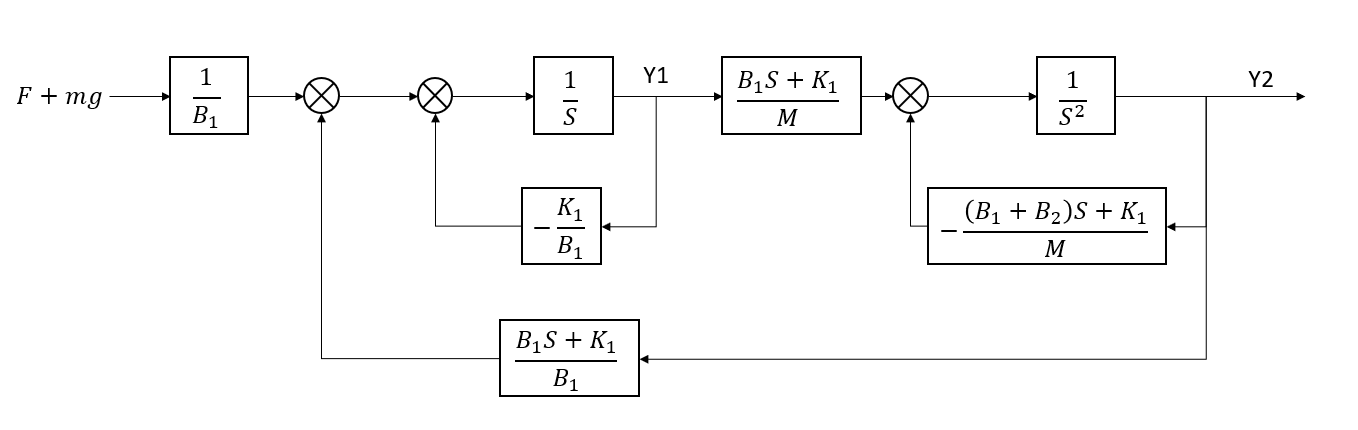
\includegraphics[width=1\textwidth]{hw3_p2bd.png} % Block diagram image.
\end{center}

\subsubsection*{Transfer Function}

For \(Y_2/F\):

\begin{align}
    M_1 &= \frac{1}{B_1} \times \frac{1}{S} \times \frac{B_1S + K_1}{M \times S^2} \\
    &= \frac{B_1S + K_1}{M B_1 S^3} \\
    \Delta_1 &= 1 \\
    \Delta &= \frac{M B_1 S^3 + M K_1 S^2 + B_1 B_2 S^2 + B_2 K_1 S}{M B_1 S^3} \\
    Y_2/F &= \frac{M_1 \Delta_1}{\Delta} = \frac{B_1 S + K_1}{M B_1 S^3 + M K_1 S^2 + B_1 B_2 S^2 + B_2 K_1 S}
\end{align}
For \(Y_1/F\):

\begin{align}
    M_1 &= \frac{1}{B_1} \times \frac{1}{S} \\
    \Delta_1 &= \frac{M S^2 + (B_1 + B_2) S + K_1}{M S^2} \\
    Y_1/F &= \frac{M_1 \Delta_1}{\Delta} = \frac{M S^2 + (B_1 + B_2) S + K_1}{M B_1 S^3 + M K_1 S^2 + B_1 B_2 S^2 + B_2 K_1 S}
\end{align}


\newpage
\section*{Problem \#3}
From the figure below, find the following:
\newline
\begin{center}
    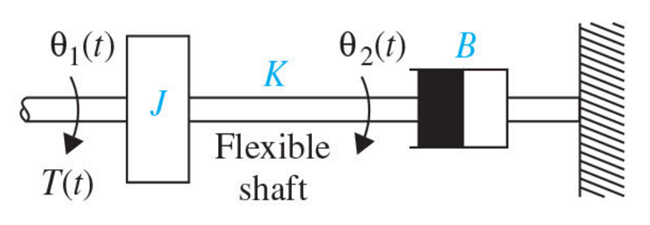
\includegraphics[width=0.6\textwidth]{hw3_p3.png}
\end{center}

\begin{enumerate}
    \item Write the torque equations of the rotational systems shown.
    \item Write the state equations.
    \item Find the transfer functions \(\Theta_1(s)/T(s)\) and \(\Theta_2(s)/T(s)\) for the system.
\end{enumerate}

\subsubsection*{Solution}

\begin{align}
    J \ddot{\theta_1} &= T - K (\theta_1 - \theta_2) \\
    K (\theta_1 - \theta_2) &= B \dot{\theta_2}
\end{align}

\subsubsection*{Laplace Transform}

\begin{align}
    S^2 \theta_1 &= \frac{T}{J} - \frac{K}{J} \Theta_1 + \frac{K}{J} \Theta_2 \\
    S \theta_2 &= \frac{K}{B} \theta_1 - \frac{K}{B} \theta_2
\end{align}

\begin{center}
    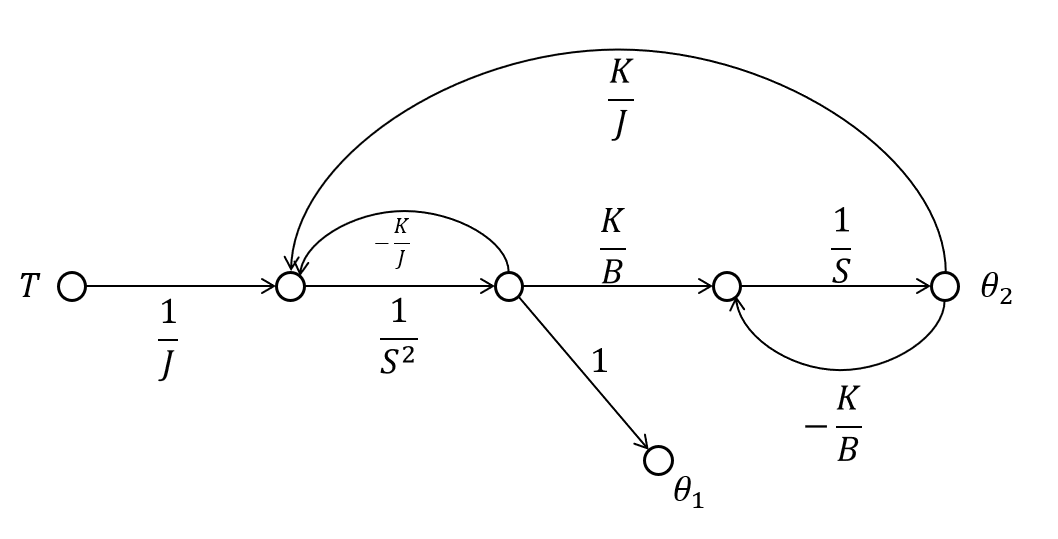
\includegraphics[width=0.9\textwidth]{hw3_p3sfg.png}
\end{center}

From the Signal Flow Graph (SFG), we have:
\begin{align}
    L_1 &= -\frac{K}{J} \times \frac{1}{S^2} \\
    L_2 &= \frac{1}{S^2} \times \frac{K}{B} \times \frac{1}{S} \times \frac{K}{J} \\
    L_3 &= \frac{1}{S} \times -\frac{K}{B}
\end{align}

Non-touching loops:
\[ L_{13} = \frac{K^2}{BJ} \times \frac{1}{S^2} \]

Given,
\[ \Delta = \dots = \frac{BJS^2 + KJS + BK}{BJS^2} \]

For \( \frac{\theta_1}{T} \):
\begin{align}
    \text{Forward path } M_1 &= \frac{1}{JS^2} \\
    \text{Path does not touch } L_3, \Delta_1 &= \frac{BS + K}{BS} \\
    \frac{\theta_1}{T} &= \frac{M_1 \Delta_1}{\Delta} = \frac{BS + K}{S(BJS^2 + KJS + BK)}
\end{align}

For \( \frac{\theta_2}{T} \):
\begin{align}
    \text{Forward path } M_1 &= \frac{1}{J} \times \frac{1}{S^2} \times \frac{K}{B} \times \frac{1}{S} \\
    \frac{\theta_2}{T} &= \frac{K}{S(BJS^2 + KJS + BK)}
\end{align}

\newpage

\section*{Problem \#4}
For the circuit shown in the figure:
\newline
\begin{center}
    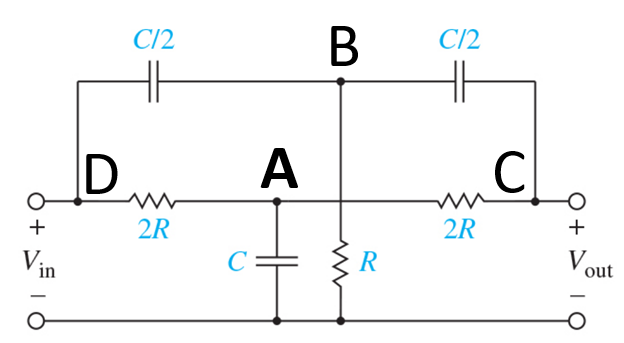
\includegraphics[width=0.7\textwidth]{hw3_p4.png}
\end{center}

\begin{enumerate}
    \item Find the dynamic equations and state variables.
    \item Determine the transfer function.
\end{enumerate}

\subsubsection*{Node Analysis}

For Node \(A\):
\begin{equation}
    i_1 + i_2 + i_3 = 0 \tag{1}
\end{equation}
For Node \(B\):
\begin{equation}
    i_4 + i_5 + i_6 = 0 \tag{2}
\end{equation}
For Node \(C\):
\begin{equation}
    i_2 + i_5 = 0 \tag{3}
\end{equation}
Given:
\begin{align*}
    i_1 &= \frac{v_{in} - e_c}{2R} \\
    i_2 &= \frac{v_{out} - e_c}{2R} \\
    e_c &= -\frac{1}{c} \int i_3 \, dt \implies i_3 = -C\dot{e}_c \\
    i_4 &= \frac{C}{2}(\dot{v}_{in} - \dot{e}_R) \\
    i_5 &= \frac{C}{2}(\dot{v}_{out} - \dot{e}_R) \\
    i_6 &= -\frac{e_R}{R}
\end{align*}
Substitute into equations (1), (2), and (3):

\begin{align*}
    \frac{v_{in} - e_c}{2R} + \frac{v_{out} - e_c}{2R} - C\dot{e}_c &= 0 \\
    \frac{C}{2}(\dot{v}_{in} - \dot{e}_R) + \frac{C}{2}(\dot{v}_{out} - \dot{e}_R) - \frac{e_R}{R} &= 0 \\
    \frac{v_{out} - e_c}{2R} + \frac{C}{2}(\dot{v}_{out} - \dot{e}_R) &= 0
\end{align*}
Which yields:

\begin{align*}
    v_{in} + v_{out} - 2e_c - 2RC\dot{e}_c &= 0 \\
    \dot{v}_{in} + \dot{v}_{out} - \frac{2}{RC} e_R - 2\dot{e}_R &= 0 \\
    v_{out} + RC\dot{v}_{out} - e_c - RC\dot{e}_R &= 0
\end{align*}

\subsubsection*{Laplace Transform}

From the Laplace transformation:
\begin{align}
    E_C &= \frac{V_{in} + V_{out}}{2(RCS + 1)} \tag{4} \\
    E_R &= \frac{RCS(V_{in} + V_{out})}{2(RCS + 1)} \tag{5} \\
    V_{out} &= \frac{RCS}{RCS + 1}E_R + \frac{1}{RCS + 1}E_C \tag{6}
\end{align}
Substituting, we obtain:
\[ \frac{V_{in}}{V_{out}} = \frac{(RCS)^2 + 1}{(RCS)^2 + 4RCS + 1} \]



\end{document}